% SPDX-FileCopyrightText: 2023 SAP SE
%
% SPDX-License-Identifier: Apache-2.0
%
% This file is part of FEDEM - https://openfedem.org

%%%%%%%%%%%%%%%%%%%%%%%%%%%%%%%%%%%%%%%%%%%%%%%%%%%%%%%%%%%%%%%%%%%%%%%%%%%%%%%%
%
% FEDEM Theory Guide.
%
%%%%%%%%%%%%%%%%%%%%%%%%%%%%%%%%%%%%%%%%%%%%%%%%%%%%%%%%%%%%%%%%%%%%%%%%%%%%%%%%

\subsection{Spring-based cam joint formulation}
\label{subs:Spring-based cam joint formulation}

Contact between the slave triad and the cam surface can be modeled using the
formulation described above in Section~\ref{subs:Cam Joint}, by introducing
non-linear springs in the two translational joint variables $\tilde u$ and
$\tilde v$ of \eqnref{eq:CamDef}, or in one of them only by using
\eqnref{eq:CamFixY} or~\eqref{eq:CamFixX}.
However, in situations with large relative separation between the slave triad
and the cam curve, or if the cam curve has sharp corners (infinite curvature),
the solution might become unstable using this formulation.

A more robust alternative is to use a purely spring-based formulation for such
contact problems\footnote{This spring-based formulation has actually been the
default formulation in Fedem since version R2.5m3.}.
This is actually a multi-master equivalent to the {\em global spring\/}
element described in Section~\ref{subs:Global spring}.
That is, it does not involve a transformation of the free variables according to
\meqsref{eq:CamDef}{eq:CamDef2}.
Instead, the stiffness and force contributions from the springs are added
directly to the slave and (some of) the master triad DOFs of the cam joint.

A set of (up to) six orthogonal joint springs (three translational and three
rotational springs) connect the slave node to the follower location on the
cam curve, i.e., the projection of the slave location onto the cam curve
along the local $x$-direction, see Figure~\ref{fig:CamSpring}.
A spring must always be present in the local $x$-direction
(the surface normal direction), otherwise no contact would be established.
In the other five directions, spring-constraining is optional.
%
\begin{figure}[b]
\begin{center}
\setlength{\unitlength}{1mm}
\begin{picture}(80,50)
\thinlines
\put(0,0){\line(1,0){80}}
\put(0,-3){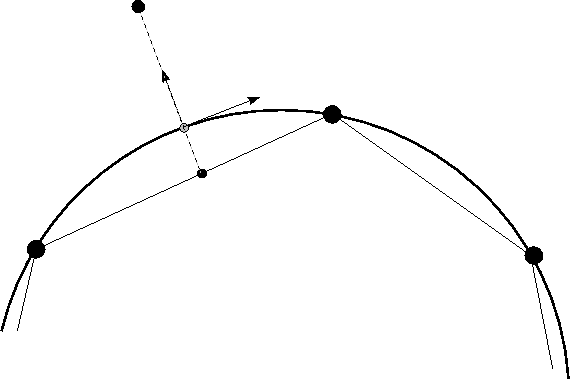
\includegraphics[width=8cm]{Figures/ContactPoint.png}}
\put(22,50){slave node; $S$}
\put(38,36){$z$}
\put(19,38){$x$}
\put(8,13){master node; \large $i$}
\put(45,29){\large $j$}
\put(70,12){\large $k$}
\put(-12,38){contact point; $C$}
\put(14,38){\vector(2,-1){10}}
\put(11,6){master secant point; $M$}
\put(44,10){\vector(-1,1){15}}
\end{picture}
\end{center}
\caption{The geometry of the spring-based cam joint.}
\label{fig:CamSpring}
\end{figure}

\remark{The remark on rotational stiffnesses in global spring elements given in
Section~\ref{subs:Global spring}, also applies to the spring-based cam joint.
Therefore, when using rotational springs, make sure they are stiff enough to
avoid large relative rotations.}

The springs are assumed located at the contact point, $C$, with rigid arms to
the slave node ($S$) and the master secant point ($M$), respectively.
Let ${\mf k}_c = \lceil k_i \rfloor$ and ${\mf f}_c = \{ f_i \}$, $i=1\ldots6$,
denote the diagonal stiffness matrix and the associated force vector of the
compound joint spring in its local system.
The contributions to the slave node are then found as
%
\begin{equation}
{\mf k}_s \;=\; {\mf T}_s{\mf k}_c{\mf T}_s^T \quad\text{and}\quad
{\mf f}_s \;=\; {\mf T}_s{\mf f}_c \quad\text{with}\quad
{\mf T}_s \;=\; \left[\begin{array}{cc}
{\mf I} & {\mf 0} \\ \widehat{\mf e}_s & {\mf I} \end{array}\right]
\end{equation}
%
where ${\mf e}_s = {\mf x}_c - {\mf x}_s$ is the eccentricity vector from the
slave node to the contact point, $C$.
Similarly, the contributions to master node $i$ are found as
%
\begin{equation}
{\mf k}_i \;=\, -f_i(\xi){\mf T}_m{\mf k}_c{\mf T}_m^T \;,\;
{\mf f}_i \;=\, -f_i(\xi){\mf T}_m{\mf f}_c \quad\text{with}\quad
{\mf T}_m \,=\, \left[\begin{array}{cc}
{\mf I} & {\mf 0} \\ \widehat{\mf e}_m & {\mf I} \end{array}\right]
\end{equation}
%
where ${\mf e}_m = {\mf x}_c - {\mf x}_m$ is the eccentricity vector from the
master secant point ($M$) to the contact point, and the function $f_i(\xi)$
is a linear interpolation function distributing the contributions to the two
closest master nodes, and is given by~\eqnref{eq:MultimasterWeight}.

The updated spring lengths in the spring-based cam joint are computed similarly
as for the global spring element of Section~\ref{subs:Global spring}.
However, for the rotational springs we now always assume zero initial angle and
deflection, regardless of the modeling configuration,
such that the computations become
%
\begin{eqnarray}
\label{eq:CamSpringLength}
{\mf l} \;=\hskip4pt \left[\; l_x \hskip6pt l_y \hskip6pt 0\;\right]^T &=&
{\mf R}_c^T({\mf x}_s - {\mf x}_c) \\
\label{eq:CamSpringAngle}
{\tf\alpha} \;=\; \left[\alpha_x \; \alpha_y \; \alpha_z\right]^T &=&
{\rm EulerZYX}({\mf R}_c^T{\mf R}_s^T{\mf R}_{s0}^T{\mf R}_{c0})
\end{eqnarray}
%
Here, ${\mf x}_s$ and ${\mf x}_c$ denote the current global position vectors of
the slave node and the contact point, respectively, whereas ${\mf R}_s$ and
${\mf R}_c$ denote the associated transformation matrices representing their
current orientation, and ${\mf R}_{s0}$ and ${\mf R}_{c0}$
are the corresponding orientations of the initial (modeling) configuration.
It also possible to assign spring properties to the local $z$-direction, and the
spring length $l_z$ is then identical to the current curve length position, $s$.

\subsubsection{Radial contact spring}

By assigning stiffness functions that have zero stiffness in a certain
deflection range around zero, and a high stiffness on both sides outside
this range, it is possible to model that the slave should remain inside
a cylindric surface along the cam curve.
However, for this cylinder to have a circular cross section (like a pipe),
the contact spring(s) should be effective in a radial coordinate system
($r,\theta$), rather than the local Cartesian system ($x,y$).

The polar spring lengths ($l_r,l_\theta$) are obtained from
\eqnref{eq:CamSpringLength} through
%
\begin{equation}
l_r \;=\; \sqrt{l_x^2+l_y^2} \quad\text{and}\quad
l_\theta \;=\; \arctan\left(\frac{l_y}{l_z}\right)
\end{equation}
%
The corresponding spring stiffnesses and forces are then applied in the radial
$r$-direction, and in the circular $\theta$-direction defined such that the
$\theta$-axis is orthogonal to both the $r$- and $z$-directions,
and ($r,\theta,z$) forms a right-handed system.
In addition, we get a geometric stiffness contribution in $\theta$-direction
of magnitude $F_r/l_r$ where $F_r$ is the computed spring force in
$r$-direction, due to the changing direction of the radial spring.

\remark{The radial contact spring must have zero stiffness for small spring
lengths or deflections.
Otherwise, the geometric stiffness term, $F_r/l_r$, will go to infinity
and cause solution instabilities.}
